% !TEX root = ../main.tex

\chapter{Appendix} % Main appendix title
\label{ch:appendix}

\section{Additional Plots}
% \begin{figure}[!ht]
% \begin{figrow}
% \item \label{row:Polynomial2_CartPole}  \raisebox{-0.5\height}{
% 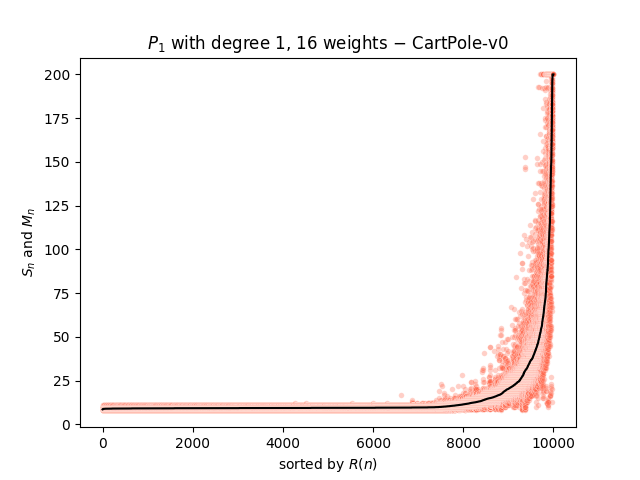
\includegraphics[width=.3\linewidth]{experiment_1/without_bias/CartPole-v0_PolynomialNN_degree_1_scatter_score}
% 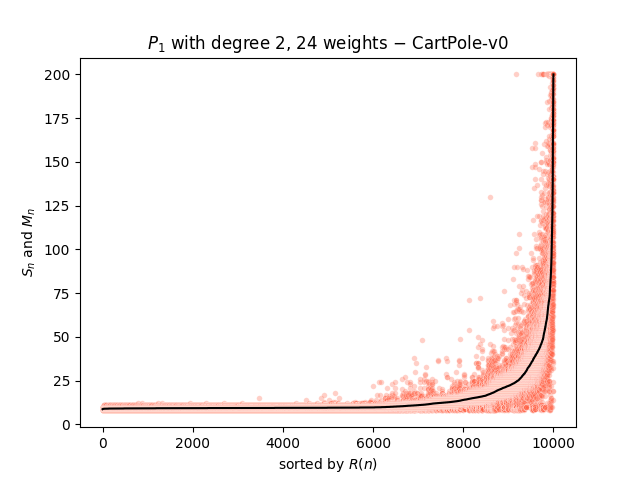
\includegraphics[width=.3\linewidth]{experiment_1/without_bias/CartPole-v0_PolynomialNN_degree_2_scatter_score}
% 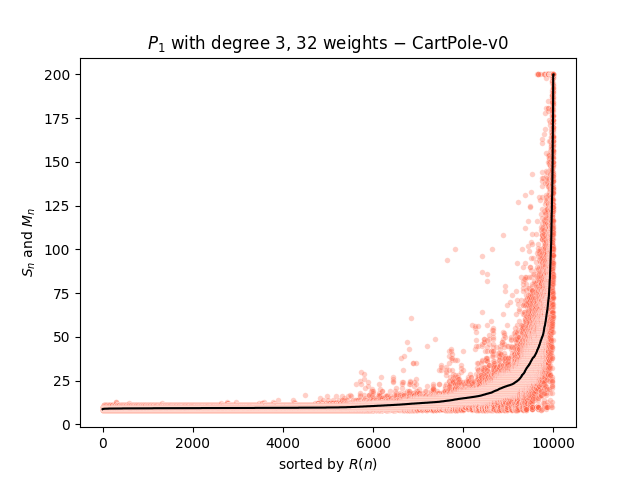
\includegraphics[width=.3\linewidth]{experiment_1/without_bias/CartPole-v0_PolynomialNN_degree_3_scatter_score}}
% \item \label{row:Polynomial2_Acrobot}  \raisebox{-0.5\height}{
% 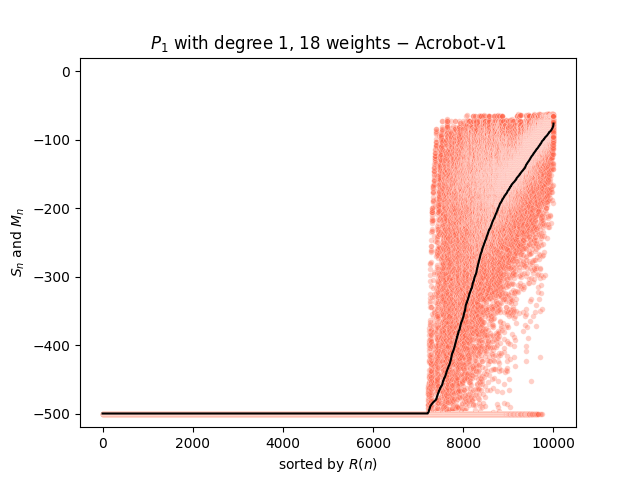
\includegraphics[width=.3\linewidth]{experiment_1/without_bias/Acrobot-v1_PolynomialNN_degree_1_scatter_score}
% 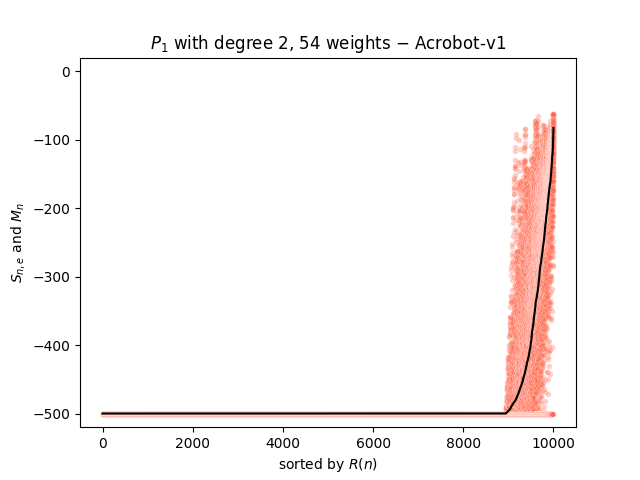
\includegraphics[width=.3\linewidth]{experiment_1/without_bias/Acrobot-v1_PolynomialNN_degree_2_scatter_score}
% 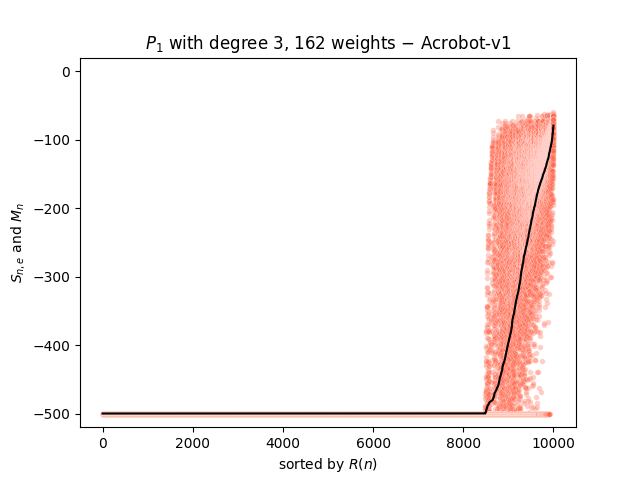
\includegraphics[width=.3\linewidth]{experiment_1/without_bias/Acrobot-v1_PolynomialNN_degree_3_scatter_score}}
% \item \label{row:Polynomial2_MountainCar}  \raisebox{-0.5\height}{
% 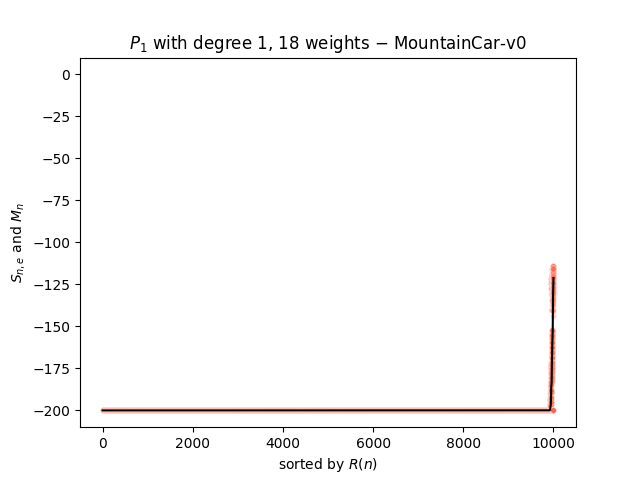
\includegraphics[width=.3\linewidth]{experiment_1/without_bias/MountainCar-v0_PolynomialNN_degree_1_scatter_score}
% 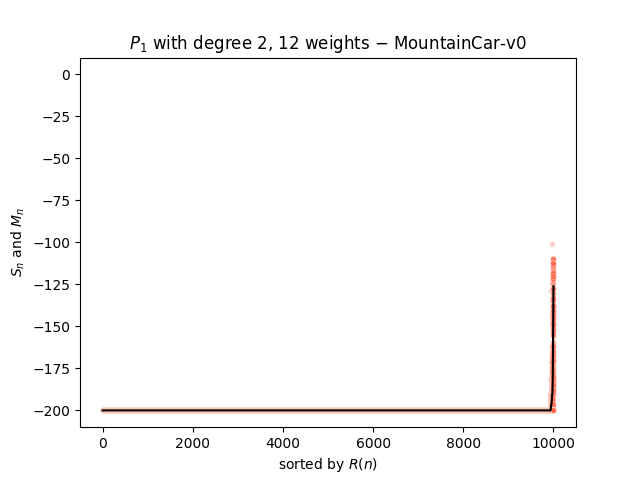
\includegraphics[width=.3\linewidth]{experiment_1/without_bias/MountainCar-v0_PolynomialNN_degree_2_scatter_score}
% 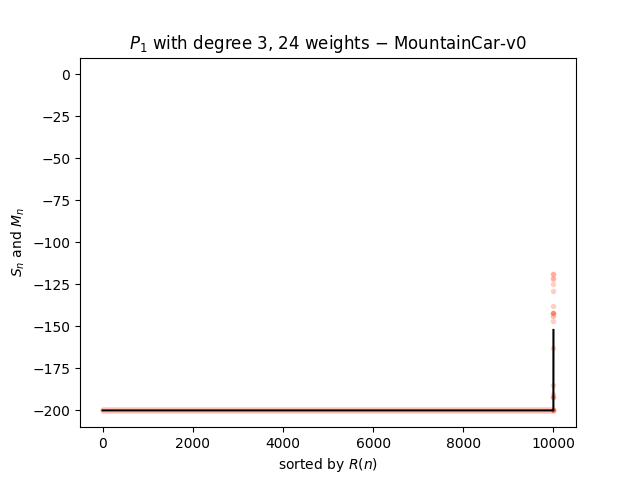
\includegraphics[width=.3\linewidth]{experiment_1/without_bias/MountainCar-v0_PolynomialNN_degree_3_scatter_score}}
% \end{figrow}
% \caption[Results for the classic control environments using polynomials]{
%   \textbf{Results for the discrete classic control environments using the polynomial model $\mathbf{P_1}$.}
%    Each row shows the results of one environment. The columns represent the different degrees of the polynomials. In these plots the model $P_1$ was used.
% }
% \label{fig:results_Polynomial2}
% \end{figure}
% The color of links can be changed to your liking using:
% {\small\verb!\hypersetup{urlcolor=red}!}, or
% {\small\verb!\hypersetup{citecolor=green}!}, or
% {\small\verb!\hypersetup{allcolor=blue}!}.
% \noindent If you want to completely hide the links, you can use:
% {\small\verb!\hypersetup{allcolors=.}!}, or even better:
% {\small\verb!\hypersetup{hidelinks}!}.
% \noindent If you want to have obvious links in the PDF but not the printed text, use:
% {\small\verb!\hypersetup{colorlinks=false}!}.
